%!TEX root = thesis.tex

\chapter{Normality test results} % (fold)
\label{cha:normality_tests}
The D'Agostino test is a suitable test for normality. This test calculates the skewness and kurtosis of the data and compares this data with the expected values from a Gaussian distribution. With this test, the null hypothesis states the data is sampled from a Gaussian distribution. This appendix contains all normality tests performed in this thesis.

\section{Priority and severity} % (fold)
\label{sec:priority_and_severity}

\subsection{Package size} % (fold)
\label{sub:norm:package_size}
The distributions of the data sets is depicted in Figure~\ref{fig:packages-density-sevcore}. Nothing can be said about the distribution of the data, except that is roughly similar shaped.  The results for the D'Agostino tests of all twelve data sets are shown in Table~\ref{tab:package-sev-core-agostino}. As can be seen, none of the $p$-values is higher than a significance level of $\alpha = 0.001$, meaning we reject the null hypothesis that the data sets follows a Gaussian distribution. For severity `normal' for the metrics NOC and SUMLOC, the D'Agostino test does not give a result. However, based on the density graph, it can be assumed the data is also not normal distributed.

\begin{figure}
        \begin{subfigure}[b]{0.5\textwidth}
                \centering
                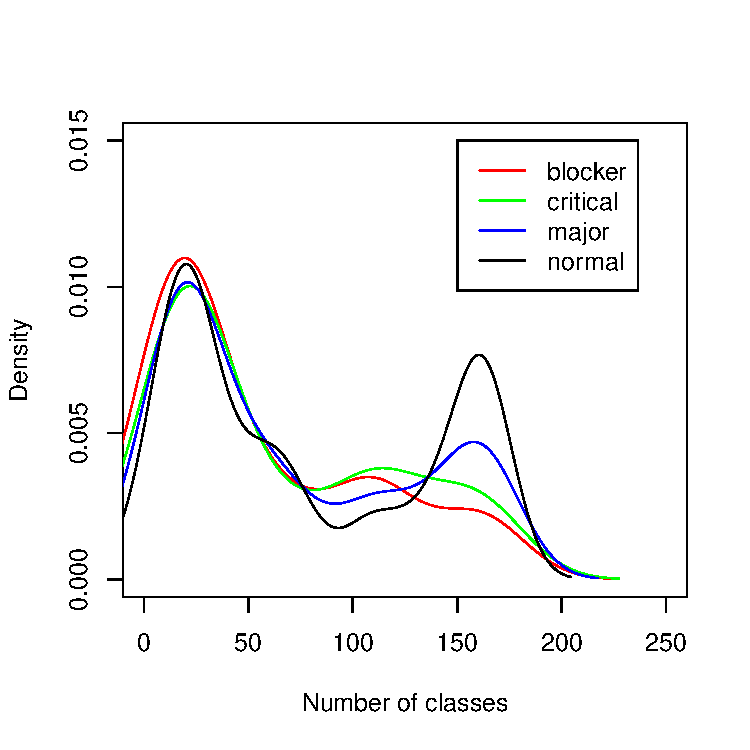
\includegraphics[width=\textwidth]{img/sev-core-noc-density.pdf}
                \caption{NOC}
                \label{fig:density-sevcore-noc}
        \end{subfigure}%
        ~ %add desired spacing between images, e. g. ~, \quad, \qquad etc. 
          %(or a blank line to force the subfigure onto a new line)
        \begin{subfigure}[b]{0.5\textwidth}
                \centering
                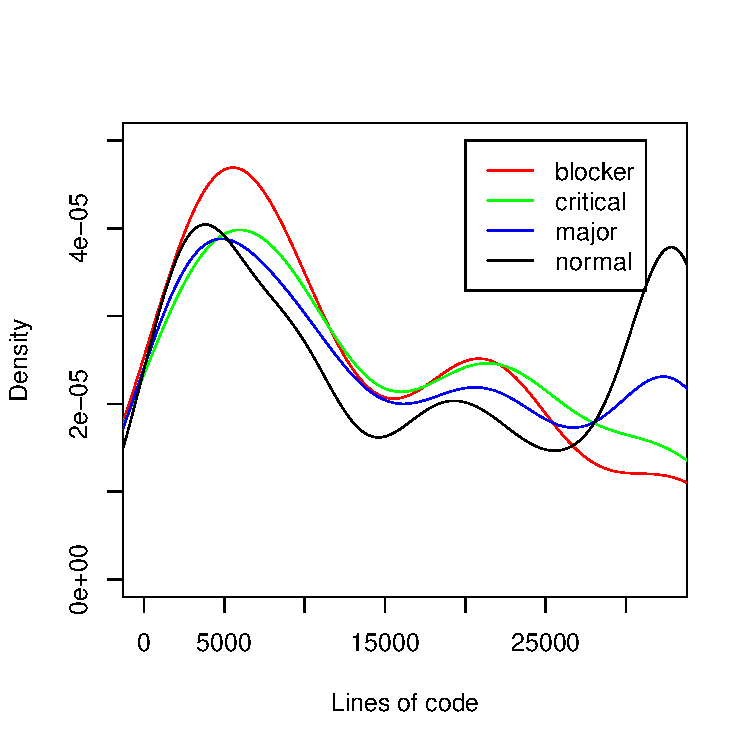
\includegraphics[width=\textwidth]{img/sev-core-sumloc-density.pdf}
                \caption{SUMLOC}
                \label{fig:density-sevcore-sumloc}
        \end{subfigure}

        \begin{subfigure}[b]{0.5\textwidth}
                \centering
                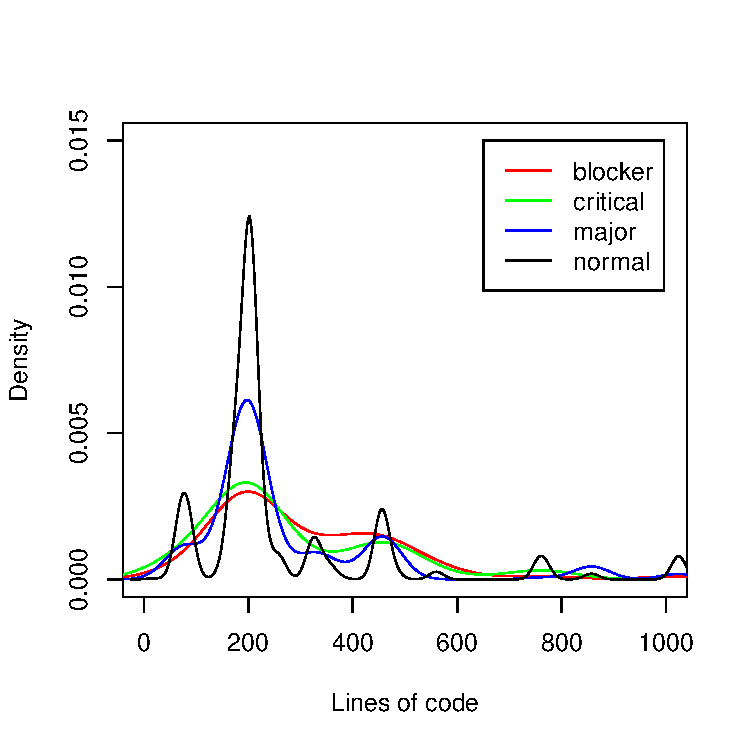
\includegraphics[width=\textwidth]{img/sev-core-avgloc-density.pdf}
                \caption{AVGLOC}
                \label{fig:density-sevcore-avgloc}
        \end{subfigure}
        \caption{Density graph for the distribution of data under investigation (jdt.core).}
        \label{fig:packages-density-sevcore}
\end{figure}

\begin{table}[!ht]\footnotesize
	\centering
	\begin{tabular}{lrl}
		\toprule
		Data set & p-value & \\
		\midrule
		NOC \\ 
		\midrule
		Blocker & $0.013$ & * \\
		Critical & $0.002$ & ** \\
		Major & $< 0.001$ & *** \\
		Normal & --\\\\
		\midrule
		SUMLOC \\
		\midrule
		Blocker & $0.026$ & * \\
		Critical & $0.002$ & ** \\
		Major & $< 0.001$ & *** \\
		Normal & -- \\\\
		\midrule
		AVGLOC \\
		\midrule
		Blocker & $< 0.001$ & *** \\
		Critical & $< 0.001$ & *** \\
		Major & $< 0.001$ & *** \\
		Normal & $< 0.001$ & *** \\
		\bottomrule
	\end{tabular} 
	\caption{D'Agostino normality test results for data under investigation. $p$-values could not be calculated for severity `normal' for metrics NOC and SUMLOC.}
	\label{tab:package-sev-core-agostino}
\end{table}

% subsection package_size (end)

\subsection{Class size} % (fold)
\label{sub:norm:class_size}
The distributions of the data sets is depicted in Figure~\ref{fig:class-sev-core-density}. Although it might look a bit like a normal distribution, the graph is zoomed in heavily. Nothing can be said about the distribution of the data, except that is roughly similar shaped. The results for all six data sets are shown in Table~\ref{tab:class-sev-core-agostino}. As can be seen, none of the p-values is higher than a significance level of $\alpha = 0.001$, meaning we reject the null hypothesis that the data sets follows a Gaussian distribution.

\begin{table}[!ht]\footnotesize
	\centering
	\begin{tabular}{lrl}
		\toprule
		Data set & p-value & \\
		\midrule
		Blocker & $< 0.001$ & *** \\
		Critical & $< 0.001$ & *** \\
		Major & $< 0.001$ & *** \\
		Normal & $< 0.001$ & *** \\
		Minor & $< 0.001$ & *** \\
		\bottomrule
	\end{tabular} 
	\caption{D'Agostino normality test results for data under investigation.}
	\label{tab:class-sev-core-agostino}
\end{table}

\begin{figure}[!ht]
	\centering
		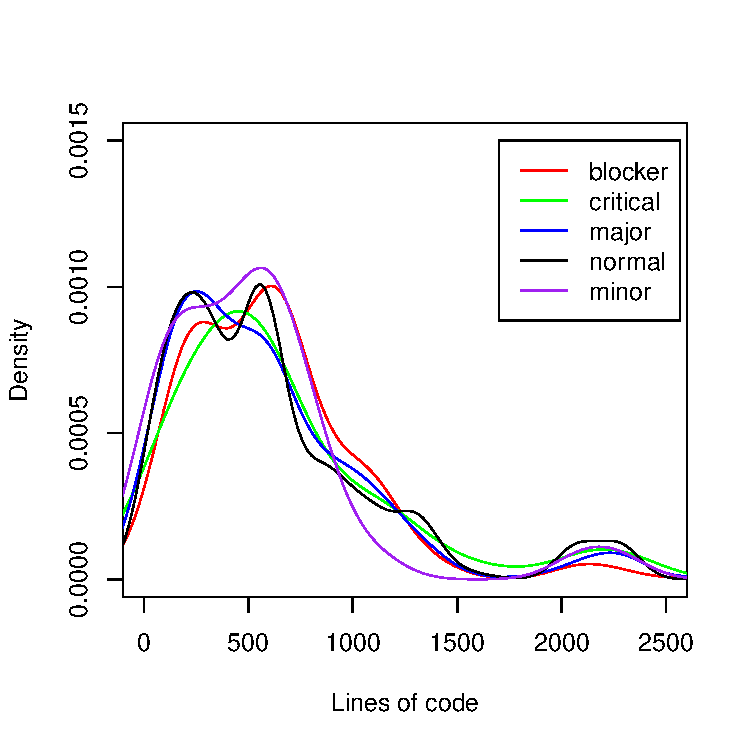
\includegraphics[width=0.7\textwidth]{img/sev-core-density.pdf}
	\caption{Density graph for the distribution of data under investigation (jdt.core).}
	\label{fig:class-sev-core-density}
\end{figure}

% subsection class_size (end)
% section priority_and_severity (end)

\section{Time-to-fix} % (fold)

\subsection{Presence of stack trace} % (fold)
\label{sub:norm:presence_of_stack_trace}
\begin{figure}[!ht]
	\centering
		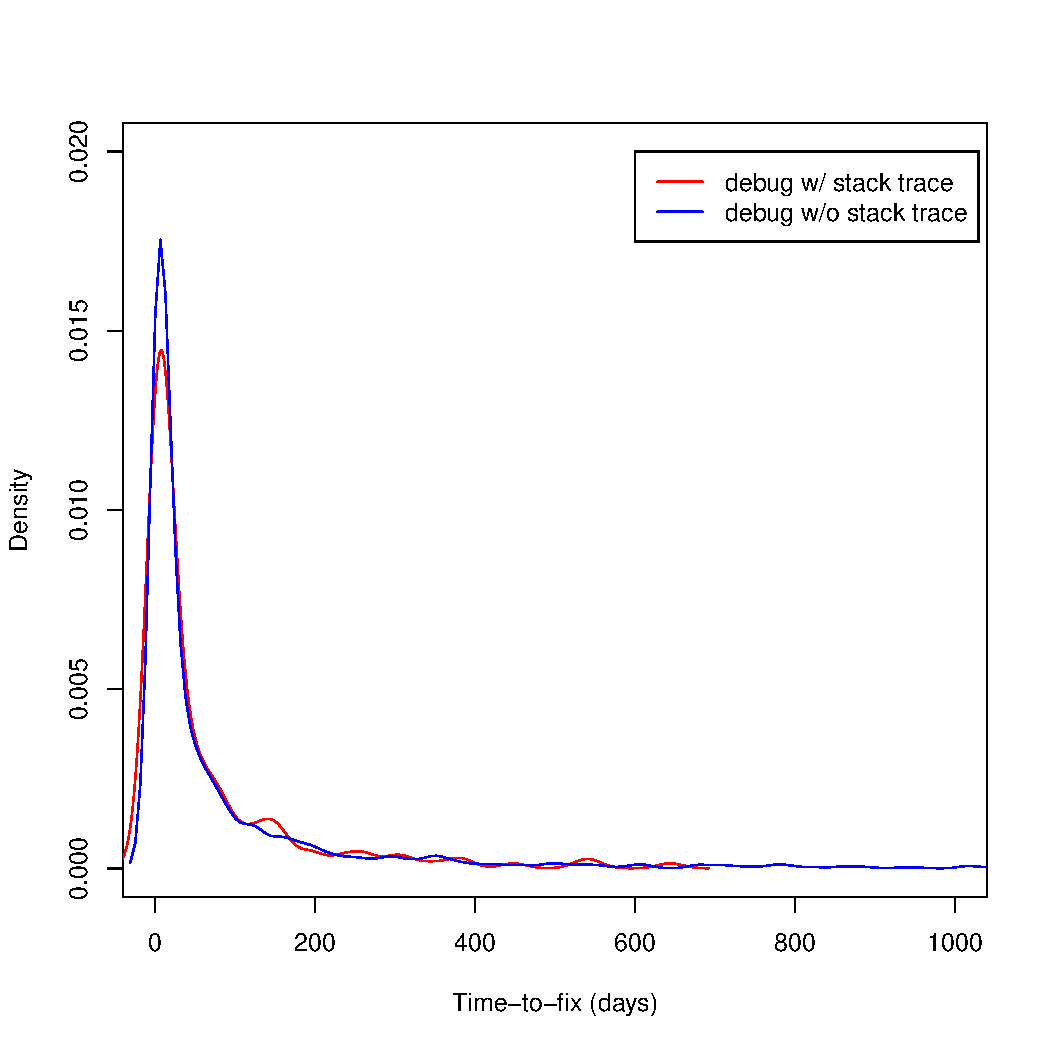
\includegraphics[width=1\textwidth]{img/ttf_with_without_stacktrace_density.pdf}
	\caption{Density plot of the data sets}
	\label{fig:ttf_density_plot}
\end{figure}

In Table~\ref{tab:ttf_stats}, the mean values are much larger than the median values. This is a characteristic of a \emph{skewed} distribution, where the skew measures the symmetry of a distribution. The skewness of the data can also be seen in Figure~\ref{fig:ttf_density_plot}, which shows the density plots of the data sets. The graph shows a Gaussian shape bell, but also shows a large tail which contains the outliers in the data. Figure~\ref{fig:ttf_density_plot} also shows the data sets have a similar shaped distribution.

These observations are a sign the data is not normally distributed. The results for all six data sets are shown in Table~\ref{tab:dagistino}. As can be seen, none of the p-values is higher than a significance level of $\alpha = 0.001$, meaning we reject the null hypothesis that the data sets follows a Gaussian distribution. 

\begin{table}[!ht]\footnotesize
	\centering
	\begin{tabular}{lrl}
		\toprule
		data set & p-value & \\
		\midrule
		jdt.debug with stack trace & $< 0.001$ & *** \\
		jdt.debug without stack trace & $< 0.001$ & *** \\
		\bottomrule
	\end{tabular} 
	\caption{D'Agostino normality test results.}
	\label{tab:dagistino}
\end{table}
% subsection presence_of_stack_trace (end)

\subsection{Stack trace position} % (fold)
\label{sub:norm:stack_trace_position}
In Table~\ref{tab:ttf_pos_stats}, the mean values are much larger than the median values. This is, again, a characteristic of a \emph{skewed} distribution. The skewness of the data can also be seen in Figure~\ref{fig:ttf_pos_stats_density}, which shows the density plots of the data sets. The graph shows a Gaussian shape bell, but also shows a large tail which contains the outliers in the data. The density plot also shows the data for jdt.core with stack traces in non-first comments has less outliers, which is of course also reflected in the overall density plot. Overall, all density plots are highly skewed and have a long tail.

These observations are a sign the data is not normally distributed. The results for all six data sets are shown in Table~\ref{tab:pos_dagistino}. As can be seen, none of the p-values is higher than a significance level of $\alpha = 0.01$, meaning we reject the null hypothesis that the data sets follows a Gaussian distribution. 

\begin{figure}[!ht]
	\centering
		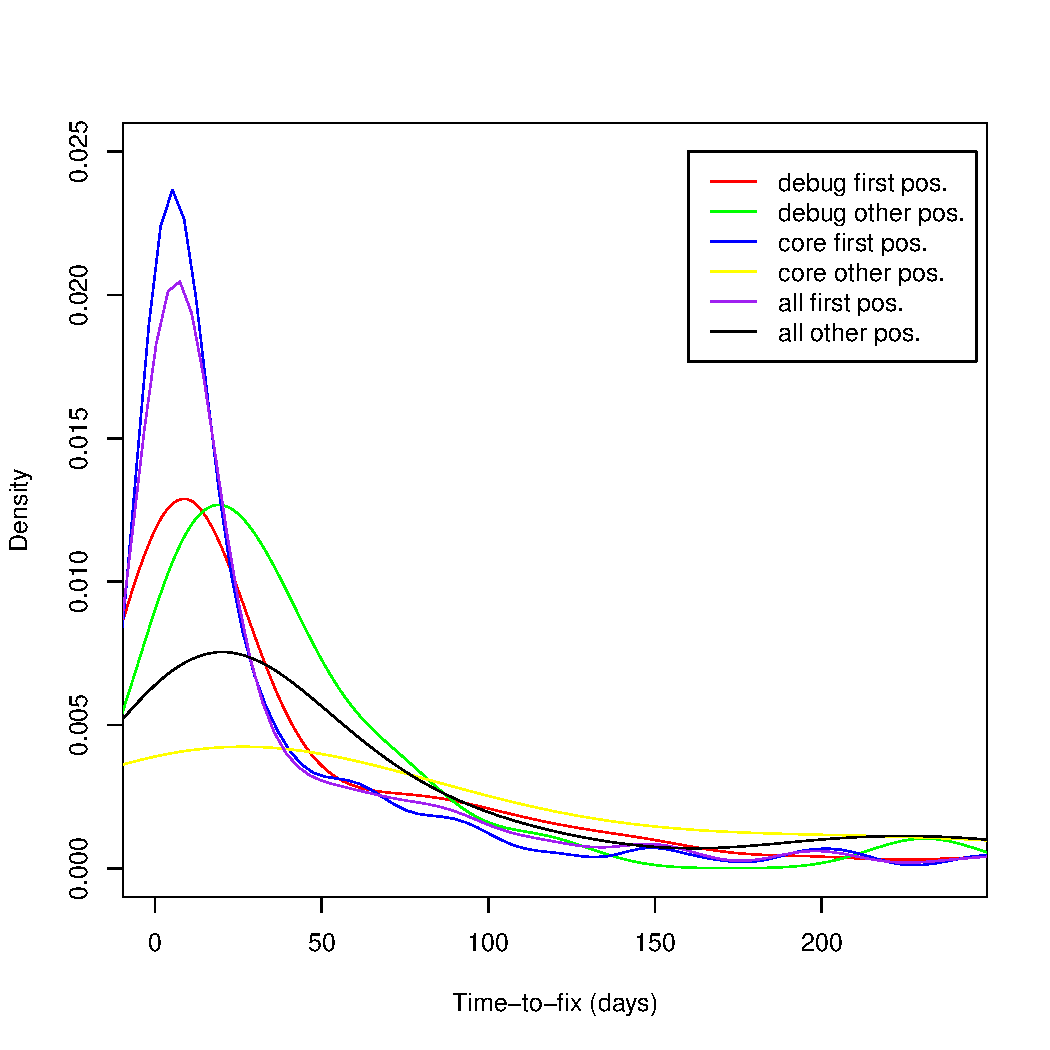
\includegraphics[width=1\textwidth]{img/ttf_stacktrace_pos_density.pdf}
	\caption{Density plot of the data sets (zoomed)}
	\label{fig:ttf_pos_stats_density}
\end{figure}

\begin{table}[!ht]\footnotesize
	\centering
	\begin{tabular}{lrl}
		\toprule
		data set & p-value & \\
		\midrule
		jdt.debug with stack traces in first comment & $< 0.001$ & *** \\
		jdt.debug with stack traces in non-first comments & $< 0.001$ & *** \\
		jdt.core with stack traces in first comment & $< 0.001$ & *** \\
		jdt.core with stack traces in non-first comments & $< 0.001$ & *** \\
		overall with stack traces in first comment & $< 0.001$ & *** \\
		overall with stack traces in non-first comments & $< 0.001$ & *** \\
		\bottomrule
	\end{tabular} 
	\caption{D'Agostino normality test results.}
	\label{tab:pos_dagistino}
\end{table}
% subsection stack_trace_position (end)

% section time_to_fix (end)

% chapter normality_tests (end)
